\section{Examples of \Glspl{name}}

Methods to detect, parse, and explain code snippets are \emph{dependent on the source language and on the desired explanation.}
In this section, we describe how we design and implement 3 \glspl{name}, highlighting the implementation decisions core to generating useful explanations.
Through these cases, we provide rationale for building custom parsers, and methods for generating usage examples and mining common usage scenarios from crowd documentation.

\subsection{CSS Selectors: Building a Custom Parser}

CSS selectors appear in tutorials that use JavaScript to select elements, stylesheets, and web scrapers that extract data from web pages.
Advanced and compound CSS selectors are named as one of five knowledge-based error types programmers frequently make when writing code in HTML and CSS, with more than half of such errors unresolved during coding tasks~\cite{park_towards_2013}.
We see them as an example of a micro-language frequently used in tandem with other languages, but infrequently described in detail when it appears.
One natural way to describe selectors is from inside out --- for example, \texttt{div a} could be described as ``select all links from all divs''.
Tokens we frequently found in online documentation included elements, IDs, classes, and properties (like \texttt{href} for links).

While we found an existing parser for CSS, this contained hundreds of lines of parse and lexer rules that covered all valid CSS, instead of the most common CSS.
Since we already knew the method that we wanted to describe CSS selectors --- from inside out --- we built a parser generator in 21 lines of an ANTLR specification that would construct a tree of elements, where each element could be marked with an ID or a class.
This provided us with a simple IR of our own specification that was simple to walk to provide the explanation we wanted.
Pseudocode for generating natural language from walking the syntax tree is shown in Figure~\ref{alg:css_traversal}.
We share examples of some of the sentences we generate in Table~\ref{tab:css_descriptions}.

\begin{figure}
\begin{algorithmic}

\Function{visit\_node}{node}
    \State clause = plural(node.element)
    \If{node has id}
        \State clause += (` with ID ' + node.id)
    \ElsIf{node has class}
        \State clause += (` of class ' + node.class)
    \EndIf
    \If{node has child}
        \State ch\_clause = visit\_node(node.child)
        \State clause = ch\_clause + `from' + clause
    \EndIf
    \State \Return clause
\EndFunction

\State
\Function{main}{parse\_tree}
    \State root\_clause = \Call{visit\_node}{parse\_tree.root}
    \State print ``This selector chooses '' + root\_clause
\EndFunction

\end{algorithmic}
\caption{Procedure for generating text description of a CSS selector by traversing the parse tree.}
\label{alg:css_traversal}
\end{figure}

\newcolumntype{S}{>{\scriptsize\arraybackslash}m{6cm}}
\newcolumntype{T}{>{\scriptsize\arraybackslash}m{9cm}}

\begin{table*}[t]
\caption{Text Generated to Explain CSS Selectors}
\label{tab:css_descriptions}
\centering
\begin{tabular}{|S|T|}
\hline
\thead{Selector} & \thead{Realized Text} \\
\hline
\texttt{div.featured a} & The selector 'div.featured a' chooses links from containers of class 'featured'. \\ \hline
\texttt{div.video-summary-data a[href\^=/video]} & The selector 'div.video-summary-data a[href\^=/video]' chooses links with URLs starting with '/video' from containers of class 'video-summary-data'. \\ \hline
\texttt{p.introduction::text} & The selector 'p.introduction::text' chooses text from paragraphs of class 'introduction'. \\ \hline
\texttt{.watch-view-count} & The selector '.watch-view-count' chooses elements of class 'watch-view-count'. \\ \hline
\texttt{.form\_box input:checked} & The selector '.form\_box input:visible' chooses visible inputs from elements of class 'form\_box'. \\ \hline
\end{tabular}
\end{table*}

\begin{figure}
\centering{
    \subfigure[\texttt{p}]{
        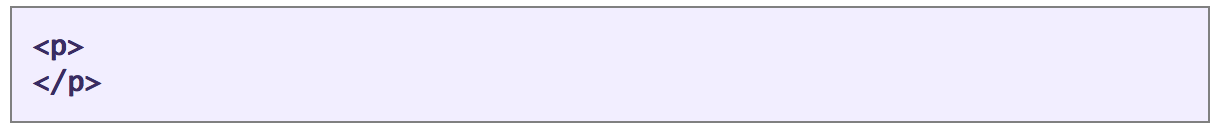
\includegraphics[width=.4\textwidth]{figures/html_p}
        \label{fig:html_p}
    }
    \subfigure[\texttt{form.myform}]{
        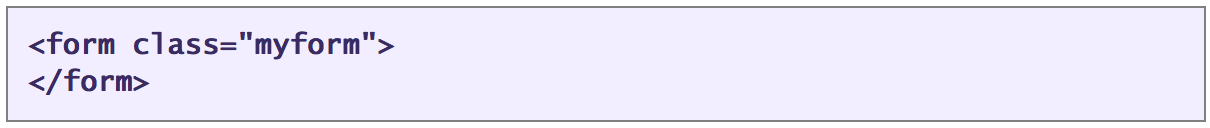
\includegraphics[width=.4\textwidth]{figures/html_form_myform}
        \label{fig:html_form.myform}
    }
    \subfigure[\texttt{table tr td}]{
        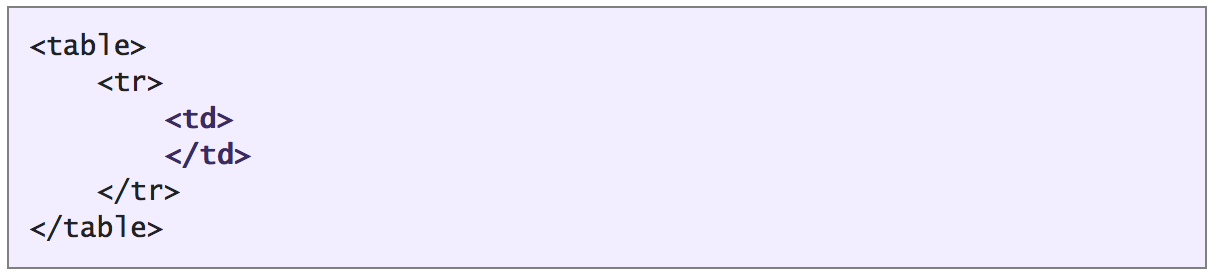
\includegraphics[width=.4\textwidth]{figures/html_table}
        \label{fig:html_table}
    }
    \subfigure[\texttt{\#first:hidden}]{
        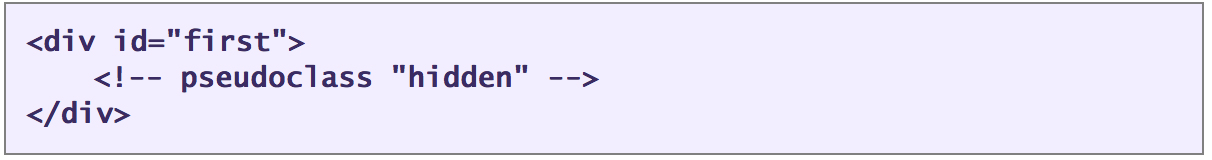
\includegraphics[width=.4\textwidth]{figures/html_pseudoclass}
        \label{fig:html_pseudoclass}
    }
    \caption{Examples of HTML DOMs that can be matched by a CSS selector, automatically generated by our CSS \gls{name}.
    Note that we bolden the font of the selected node, for example in subplot~\ref{fig:html_table}, where the selected element in the \texttt{td} nested inside a \texttt{tr} in a \texttt{table}.}
    \label{fig:fuzzy_boundaries}
}
\end{figure}

\subsection{Regular expressions: Generating Demonstrations}

Long regular expressions are cryptic even for expert readers to understand.
We expect that in some contexts, providing readable examples of what strings will satisfy and fail to satisfy these patterns could help with comprehension of the regular expressions.
While we have yet to integrate regular expressions into a \gls{name} server, we describe how we automatically generate examples of readable strings that satisfy regular expression patterns.

Given a regular expression, we parse a tree of branches, repetitions and literals.
For each repeated group (not just a character) (* or +), we generate it exactly once to make sure that the group appears in the original best example.
We print any literal exactly as it appears in the pattern.
For each branch, we choose one of the paths to render.
Whenever we have a repeated sequence of alphanumeric characters (repeated by + or *), we choose a dictionary word 4-6 letters in length.
If the character class contains symbols or numbers, we insert 2 random non-alphabetic characters.
In the future, we would like to implement in-place editors of regular expressions that enables real-time updating of these examples and checking user-defined test patterns.

\subsection{\texttt{wget}: Mining Higher-Level Meaning of Tokens}

\begin{figure}
\centering{
    \subfigure[A trivial \texttt{wget} command and an automatically-generated explanation of what it does.]{
        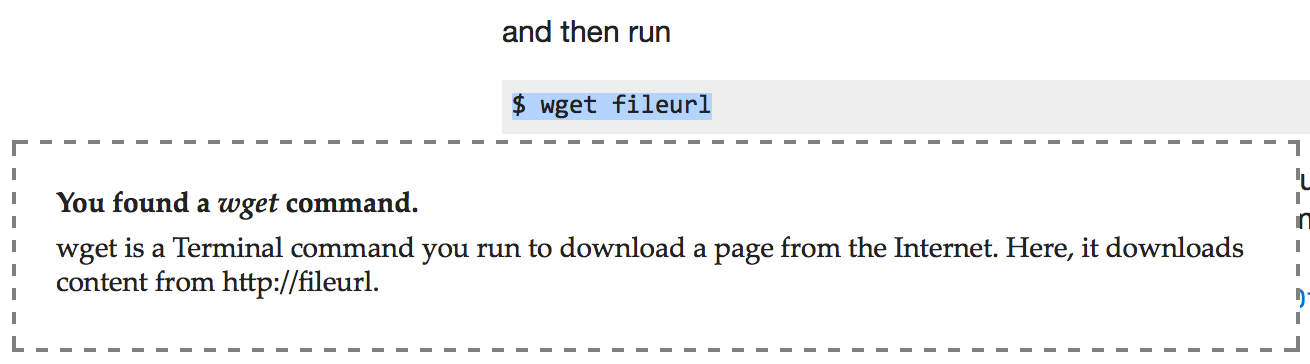
\includegraphics[width=.4\textwidth]{figures/wget_trivial}
        \label{fig:wget_trivial}
    }
    \subfigure[A complex, multi-level explanation of \texttt{wget} comprises three parts.
        \emph{(a)} An introduction to the command.
        \emph{(b)} A meaningful description of what this combination of options does at a high level.
        \emph{(c)} A review of the meaning and values of each of the options.
    ]{
        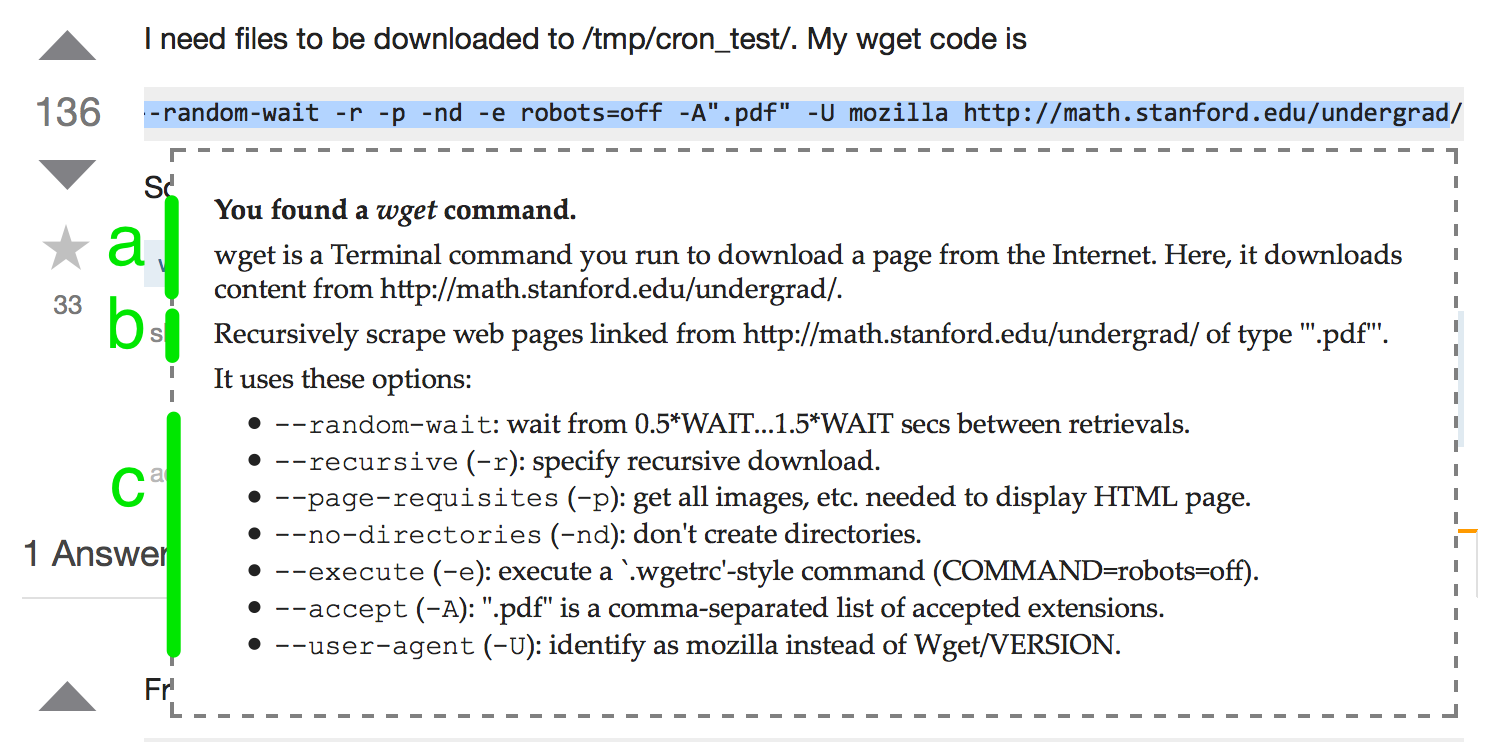
\includegraphics[width=.4\textwidth]{figures/wget_complex_explained}
        \label{fig:wget_trivial}
    }
    \caption{Descriptions of \texttt{wget} command lines, automatically generated by our \texttt{wget} \gls{name}.
        We show both a trivial and a complex example of the explanations generated.}
    \label{fig:fuzzy_boundaries}
}
\end{figure}

\newcolumntype{L}{>{\scriptsize\arraybackslash}m{5cm}}
\newcolumntype{C}{>{\tiny\arraybackslash}m{4cm}}
\newcolumntype{R}{>{\scriptsize\arraybackslash}m{6cm}}

\begin{table*}[t]
\caption{Templates for Describing Combinations of wget options}
\label{tab:wget_combos}
\centering
\begin{tabular}{|L|C|R|}
\hline
\thead{Template} & \thead{Command} & \thead{Realized Text} \\
\hline
Recursively scrape web pages linked from \{url\} of type '\{accept\}', following links \{level\} times. &
\texttt{wget -l3 -A '*.jpg' \urltarget{}} & 
Recursively scrape web pages linked from http://\urltarget{} of type '*.jpg', following links 3 times. \\
\hline
Authenticate at {url} with username '{user}' and password '{password}'. &
\texttt{wget --user andrew 
--password mypass \urltarget{}} & 
Authenticate at http://\urltarget{} with username 'andrew' and password 'mypass'. \\
\hline
\end{tabular}
\end{table*}

Command lines arguments are short for speed of typing, but recalling what each one does can be tricky.
\andrew{There's a reference we can find the Inky paper.}
\texttt{wget} has around 100 command line arguments, making it impractical to remember what each individual one means, particularly if its short flag is used instead of its full name.

We detect lines of \texttt{wget} by stripping whitespace and potential PS1 \marti{??} tokens from the start of lines, and then seeing if the line begins with `wget'.
We pass detected lines to modified wget source code, which processes the arguments and outputs them as plaintext that we can read via Python.

We noticed that for wget, the meaning of a command is often more than the sum of the value of its arguments.
For examples, when \texttt{--user} and \texttt{--password} are used together, the caller is authenticating to access a restricted resource.
By using \texttt{-A} and \texttt{-r} together, users can recursively scrape a site for files of a certain type.

Here, we propose a workflow for extracting common use cases for commands with multiple arguments that should be explained as a unit instead of a `sum of parts'.
Using StackOverflow, developers can mine combinations of parameters that mean more than the sum of individual parameters.
Through a preliminary effort with \texttt{wget}, we showed that one can find reasonable combinations of arguments that should be described together by scraping and observing frequent combinations of arguments from commands scraped from StackOverflow \marti{Who is "one" and what is "reasonable"? (need to be more precise).} (Figure~\ref{fig:wget_arguments}).
For example, for \texttt{wget}, the combination of the \texttt{-r}, \texttt{-l<level>}, \texttt{-A<ext>}, and \texttt{-e robots=off} tags suggest that a user is about to scrape a destination URL recursively to depth level \texttt{l} for files of type \texttt{A}, without following the recommended etiquette for crawler \texttt{robots}.

Using this procedure, we can create explanations like those in (Figure~\ref{fig:so_wget_explanation}). \marti{Weird figure numbering again, and the figure is too small to see.}
An initial description may just contain an overview of what the command does as a whole, inferred from the combination of arguments.
However, asking for information can provide a detailed breakdown of how each option affects the execution of the command.

\begin{figure}
\centering{
    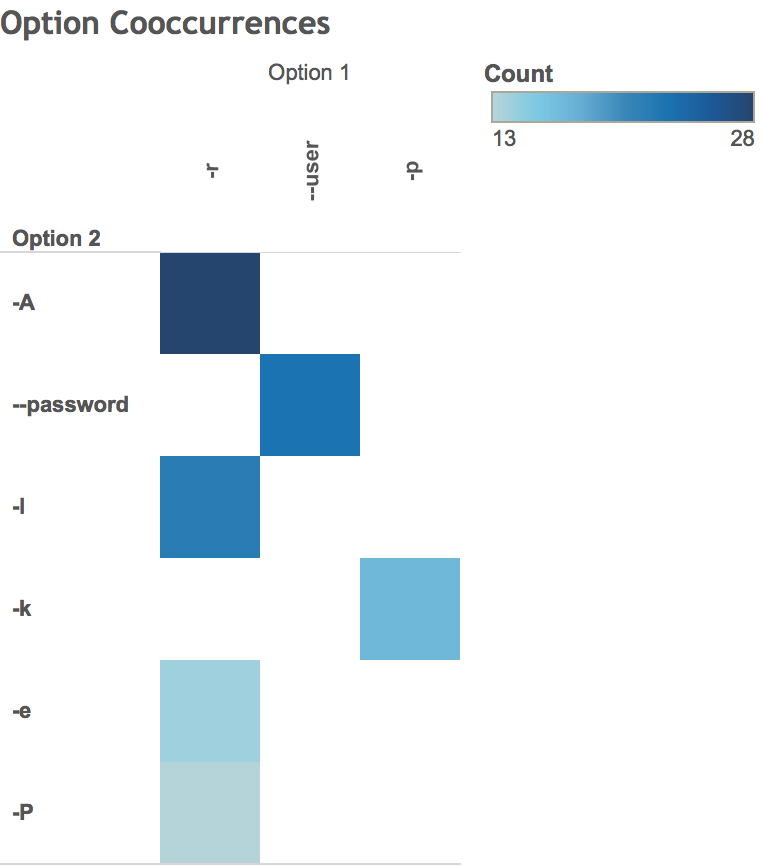
\includegraphics[width=.3\textwidth]{figures/wget_arguments}
}
\caption{\texttt{wget} arguments that frequently co-occur in uses of \texttt{wget} in StackOverflow questions. \andrew{A table would may be more readable here.}}
\label{fig:wget_arguments}
\end{figure}
